\documentclass[11pt,a4paper]{article}
\usepackage[T1]{fontenc}
\usepackage[margin=25mm]{geometry}
\usepackage{graphicx}
\usepackage{booktabs}
\usepackage{amsmath}
\usepackage{amssymb}
\usepackage{xcolor}
\usepackage{fancyhdr}
\usepackage[hidelinks]{hyperref}
\usepackage{titlesec}
\titleformat{\section}{\large\bfseries}{\thesection}{0.6em}{}
\setlength{\parskip}{0.35em}
\setlength{\parindent}{0pt}
\pagestyle{fancy}\fancyhf{}
\fancyhead[L]{\small Per-task gate threshold fit --- Qwen2.5-Omni-7B on OmniPro Online}
\fancyhead[R]{\small\thepage}
\renewcommand{\headrulewidth}{0.4pt}
\newcommand{\WITHHELD}{\textsc{withheld}}
% This report is dense with unbreakable \texttt identifiers -- gate_strategy,
% cfg.gate_high_thr, task_refractory_s -- any one of which can overflow a line
% that TeX cannot hyphenate. \sloppy trades a little inter-word stretch for a
% guarantee of no overfull boxes, which is the right trade for an internal
% record whose text changes every time the numbers do.
\sloppy
\begin{document}

\begin{center}{\LARGE\bfseries Per-task gate threshold fit for Qwen2.5-Omni-7B}\\[2mm]{\large Technical progress report --- through pass 2}\\[3mm]{\small built 2026-08-30 19:20 from the run tree at\\\texttt{/iopsstor/scratch/cscs/dthapa/system3\_qwem\_omni\_8\_28/omni\_thr\_fit}}\end{center}
\vspace{3mm}
\suppressfloats[t]

\section*{Executive summary}

This report covers a per-task fit of the output gate of a three-thread
proactive streaming pipeline built on \textbf{Qwen2.5-Omni-7B} (vision $+$ audio),
evaluated on \textbf{OmniPro Online} (2{,}700 samples, 9 tasks $\times$ 300).
The research question is \emph{when should a streaming model speak}, and the
object under study is the output gate: at every tick the controller reads
$p_\mathit{hit}=P(\text{true})$ off the logits and decides whether to emit.

\textbf{Where the run stands.} Pass 1 is complete (1410/1410 samples, 94/94 cells). Pass 2 is at 100.0\% (675/675 samples, 45/45 cells), with 0 samples outstanding. Stage 3 --- the full 2{,}700-sample evaluation --- has not started, and is roughly 72\% of the total compute for the study.

\textbf{The headline result is negative, and it is the deliverable.}
Five findings, each measured and each with its evidence file, converge on one
conclusion: \emph{the gate has one identifiable degree of freedom, not nine.}
Two of them are outright defects in the shipped system that made the nominal
per-task thresholds inert. The remaining three establish that $p_\mathit{hit}$
does not rank event-adjacent ticks above quiet ones, that the per-task fit does
not survive its own bootstrap, and that nine fitted thresholds do not beat a
single global one at a level this data can resolve.

\textbf{Honesty rules in force.} \texttt{time\_f1} is judge-free (a
$\pm3$\,s greedy one-to-one match) and is reported everywhere. \texttt{content\_acc}
and \texttt{joint\_f1} require an LLM judge; no judge endpoint is currently
reachable, so those metrics are \WITHHELD{} throughout --- never estimated, and
never rendered as a dash that could be read as zero. The evaluation is not
bit-reproducible; \textbf{$\Delta$F1 below 0.03 is treated as noise.}

\begin{table}[t]\centering\caption{Sample-level completion of the two fit passes, recounted from the banked predictions at build time. A cell is one (task, threshold) pair over the 15 frozen videos.}\label{tab:progress}
\begin{tabular}{lrrrr}\toprule
pass & banked & target & \% & cells complete \\\midrule
Pass 1 (coarse) & 1410 & 1410 & 100.0\% & 94/94 \\
Pass 2 (refine) & 675 & 675 & 100.0\% & 45/45 \\
\bottomrule\end{tabular}\end{table}


\begin{table}[t]\centering\caption{Pass-2 completion per task. The tail is not uniform: it concentrates on the tasks whose frozen videos are longest, because a lane can only claim a shard whose samples fit inside its remaining wall-clock.}\label{tab:p2tail}
\begin{tabular}{lrrrc}\toprule
task & banked & target & \% & left \\\midrule
cumulative\_counting & 75 & 75 & 100.0\% & $\checkmark$ \\
dedup\_counting & 75 & 75 & 100.0\% & $\checkmark$ \\
event\_narration & 75 & 75 & 100.0\% & $\checkmark$ \\
explicit\_target\_grounding & 75 & 75 & 100.0\% & $\checkmark$ \\
instant\_event\_alert & 75 & 75 & 100.0\% & $\checkmark$ \\
realtime\_state\_monitor & 75 & 75 & 100.0\% & $\checkmark$ \\
semantic\_condition\_alert & 75 & 75 & 100.0\% & $\checkmark$ \\
sequential\_step\_instruction & 75 & 75 & 100.0\% & $\checkmark$ \\
snapshot\_counting & 75 & 75 & 100.0\% & $\checkmark$ \\
\bottomrule\end{tabular}\end{table}


\section{The system under test}

Three threads share one KV cache. The \emph{ingester} decodes video at
1\,fps and audio in 2\,s chunks and appends to the cache; the \emph{controller}
reads $p_\mathit{hit}$ every tick and decides whether to speak; the \emph{writer}
produces the utterance when it does. The quiet path costs zero decode steps ---
$p_\mathit{hit}$ is read straight off the logits at a boolean slot, which is what
makes a tick-rate gate affordable at all.

\textbf{The gate is three coupled knobs, never one:} the threshold
\texttt{hit\_threshold}, the mode \texttt{edge} vs.\ \texttt{level}, and the
refractory period \texttt{refractory\_s}. Quoting the configuration file itself:
\emph{using the threshold without its mode and refractory does not reproduce it.}
Section~\ref{sec:f2} shows this empirically --- the size of the first-tick defect
scales with the refractory length, so the two cannot be fitted separately.

\section{Experimental design}

The fit runs on a \textbf{frozen 5\% all-audio subset}: 15 videos per
task, fixed by id before any threshold was tried, so every cell in every pass
scores the same video set and all comparisons are paired. A \emph{cell} is one
(task, threshold) pair evaluated over those 15 videos. Pass 1 sweeps a coarse
10-point grid; pass 2 refines around each task's pass-1 pick.

Two design choices matter for every number in this report.
\textbf{Pooling} is micro-averaged over tp/fp/fn exactly as
\texttt{metrics.aggregate} does it --- a mean of per-sample F1 ratios would let a
video with one ground-truth event outvote a video with thirty.
\textbf{Bootstrap resampling is over videos}, never over ticks or events: ticks
within a video are serially correlated through the shared KV cache, so resampling
them would manufacture significance out of that correlation.

Scoring is \texttt{omniprofast/metrics.py}, used unmodified. The harness
spins up the real pipeline and captures its emissions rather than reimplementing
it; a second implementation of the metric would be a second set of bugs.

\section{Findings}

\subsection{Finding 1 --- the shipped \texttt{hit\_threshold} was inert}

Under the shipped \texttt{gate\_strategy="hysteresis"} the fire test
compares \texttt{p\_hit} against \texttt{cfg.gate\_high\_thr} --- a fixed
\emph{global} 0.5. The per-task
\texttt{hit\_threshold} therefore decided only whether an answer was
\emph{decoded}, not whether the gate fired. Across the completed 2{,}700-sample
phase-A run --- 581{,}403 ticks, 50{,}433 fires --- \textbf{not one fire occurred
below $p_\mathit{hit}=0.500$}, so the four tasks configured at or below 0.5 were
all effectively running at 0.5 and their configured values were dead code.
\texttt{task\_gate\_modes} and \texttt{task\_refractory\_s} were read nowhere at
all. The fit tree replaces this with \texttt{gate\_strategy="fitted"}, which
actually consults all three knobs.

\subsection{Finding 2 --- the first tick is a spurious rising edge}\label{sec:f2}

$p_\mathit{hit}$ is high on the \emph{first tick of every video}: the
model answers the boolean from the prompt before it has seen anything
($\geq0.05$ for 98--100\% of phase-A samples in every task, median 0.34--0.64).
Seeding \texttt{prev\_above=False} made that tick a rising edge, and on a task
with a long refractory the spurious fire consumed the video's only emission ---
every \texttt{instant\_event\_alert} sample emitted once, at video time 1.0\,s,
against ground truth at 26--98\,s.

The fix is definitional rather than a tuned guard: an edge requires a
predecessor, so \texttt{prev\_above} starts \texttt{None}. Table~\ref{tab:firsttick}
shows the effect size tracking the refractory --- large on the long-refractory
tasks, $\pm0.001$ on the short ones. Applied to the live gate and to all five
offline replays.

\begin{table}[t]\centering\small\caption{The first-tick defect. \emph{as-is} seeds \texttt{prev\_above=False}, making tick 0 a rising edge; \emph{edge1} requires a predecessor (\texttt{prev\_above=None}). The size of the effect tracks the refractory length, which is why the two knobs cannot be fitted independently.}\label{tab:firsttick}
\begin{tabular}{lrrrrr}\toprule
task & as-is F1 & thr & edge1 F1 & thr & $\Delta$ \\\midrule
cumulative\_counting & 0.2505 & 0.45 & 0.2512 & 0.35 & +0.0007 \\
dedup\_counting & 0.2180 & 0.55 & 0.2171 & 0.55 & -0.0009 \\
event\_narration & 0.2408 & 0.25 & 0.2408 & 0.25 & +0.0000 \\
explicit\_target\_grounding & 0.0813 & 0.85 & 0.0844 & 0.85 & +0.0031 \\
instant\_event\_alert & 0.0636 & 0.85 & 0.0751 & 0.85 & +0.0115 \\
realtime\_state\_monitor & 0.2368 & 0.05 & 0.2368 & 0.05 & +0.0000 \\
semantic\_condition\_alert & 0.1973 & 0.05 & 0.1973 & 0.05 & +0.0000 \\
sequential\_step\_instruction & 0.4136 & 0.05 & 0.4136 & 0.05 & +0.0000 \\
snapshot\_counting & 0.0535 & 0.85 & 0.0900 & 0.05 & +0.0365 \\
\bottomrule\end{tabular}\end{table}


\begin{table}[t]\centering\small\caption{Offline replay of the refractory knob at the shipped threshold. The gains are inside the 0.03 noise band on every task, which is the empirical reason the three gate knobs are reported as one coupled operating point rather than fitted one at a time.}\label{tab:refractory}
\begin{tabular}{lrrrrr}\toprule
task & ship $r$ & F1 & best $r$ & F1 & gain \\\midrule
cumulative\_counting & 7 & 0.2512 & 5 & 0.2561 & +0.0049 \\
dedup\_counting & 5 & 0.2171 & 7 & 0.2282 & +0.0111 \\
event\_narration & 7 & 0.2408 & 7 & 0.2408 & +0.0000 \\
explicit\_target\_grounding & 300 & 0.0844 & 60 & 0.0962 & +0.0118 \\
instant\_event\_alert & 600 & 0.0751 & 20 & 0.1086 & +0.0334 \\
realtime\_state\_monitor & 7 & 0.2368 & 7 & 0.2368 & +0.0000 \\
semantic\_condition\_alert & 10 & 0.1973 & 7 & 0.2003 & +0.0031 \\
sequential\_step\_instruction & 7 & 0.4136 & 7 & 0.4136 & +0.0000 \\
snapshot\_counting & 600 & 0.0900 & 20 & 0.0956 & +0.0056 \\
\bottomrule\end{tabular}\end{table}


\subsection{Finding 3 --- $p_\mathit{hit}$ is uninformative about \emph{when}}

This is the finding that reframes the whole study. On the pass-1 tasks
with a complete reference cell, \textbf{AUC is near chance and every 95\%
confidence interval contains 0.5}. Three innocent explanations were excluded
before reporting it as a property of the model:

\begin{itemize}
\item \textbf{A clock offset} between the log's video timestamp and the
benchmark's trigger time. Swept $\pm10$\,s: no peak anywhere, so there is no
constant misalignment hiding an informative score.
\item \textbf{Too tight a tolerance}, if the model anticipates or lags events.
Re-run at $\pm10$\,s: unchanged.
\item \textbf{A degenerate score} pinned at one value. Excluded by the
distribution --- $p_\mathit{hit}$ spans 0.000--0.997 with 232--284 distinct
values and an interquartile range of 0.2--0.7.
\end{itemize}

Independently and through a separate code path, per-task \emph{precision
is flat across the entire threshold grid while recall falls} --- firing less often
buys no precision, which is exactly what an AUC of 0.5 predicts. One task,
\texttt{semantic\_condition\_alert}, comes out \emph{below} chance and falls
monotonically as the offset goes positive: its confidence is systematically lower
near an event.

The claim this supports is ``indistinguishable from chance at
$n=15$ videos per task'', never ``proven to be exactly chance''. Re-running the
same audit against stage 3 would give $n=300$.

\begin{table}[t]\centering\small\caption{Does $p_\mathit{hit}$ rank event-adjacent ticks above quiet ones? \emph{AUC best} is the highest AUC any clock offset in $\pm10$\,s or tolerance in $\{3,10\}$\,s could buy: a merely misaligned score would peak well above its zero-offset value, and none does. The $p_\mathit{hit}$ range and distinct-value count exclude the third innocent explanation, a degenerate score.}\label{tab:perception}
\begin{tabular}{lrrrrlr}\toprule
task & vid & ticks & AUC@0 & AUC best & $p_\mathit{hit}$ range & distinct \\\midrule
cumulative\_counting & 15 & 2833 & 0.469 & 0.509 & 0.003--0.997 & 284 \\
explicit\_target\_grounding & 15 & 2947 & 0.512 & 0.512 & 0.000--0.985 & 232 \\
instant\_event\_alert & 15 & 4047 & 0.551 & 0.551 & 0.001--0.990 & 247 \\
semantic\_condition\_alert & 15 & 3323 & 0.431 & 0.487 & 0.002--0.991 & 253 \\
snapshot\_counting & 15 & 3703 & 0.526 & 0.542 & 0.001--0.995 & 280 \\
\bottomrule\end{tabular}\end{table}


\begin{figure}[t]\centering
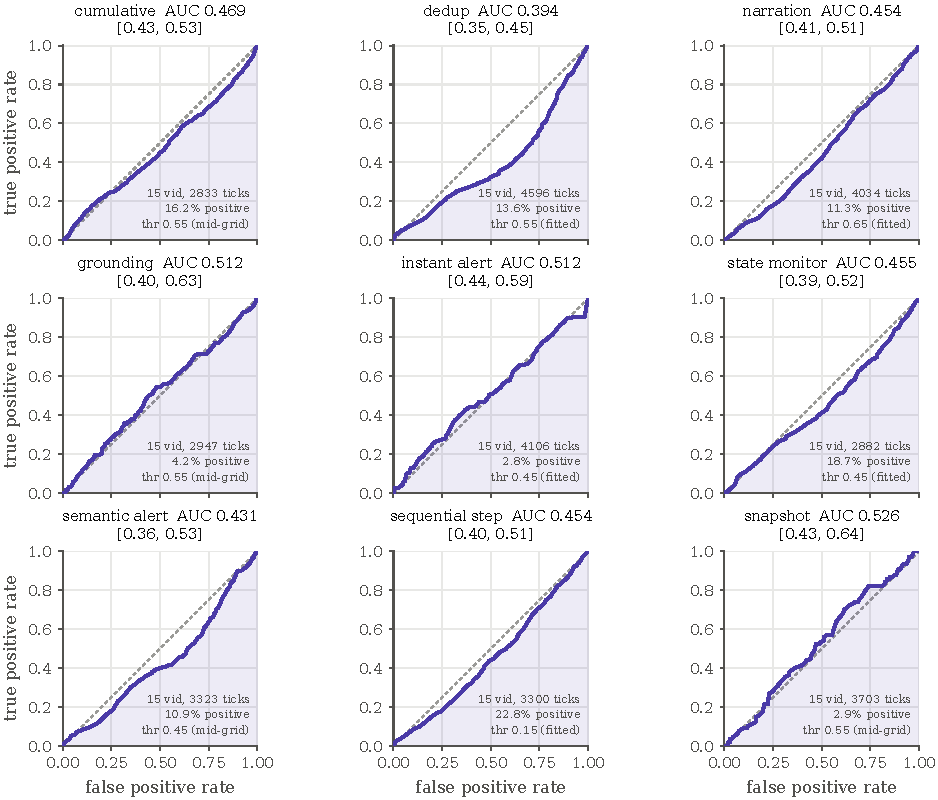
\includegraphics[width=0.92\linewidth]{../figs/fig2_roc.pdf}
\caption{ROC per task at the operating point. The diagonal is chance; every curve hugs it. This is the picture behind Table~\ref{tab:perception}.}\label{fig:roc}\end{figure}


\begin{figure}[t]\centering
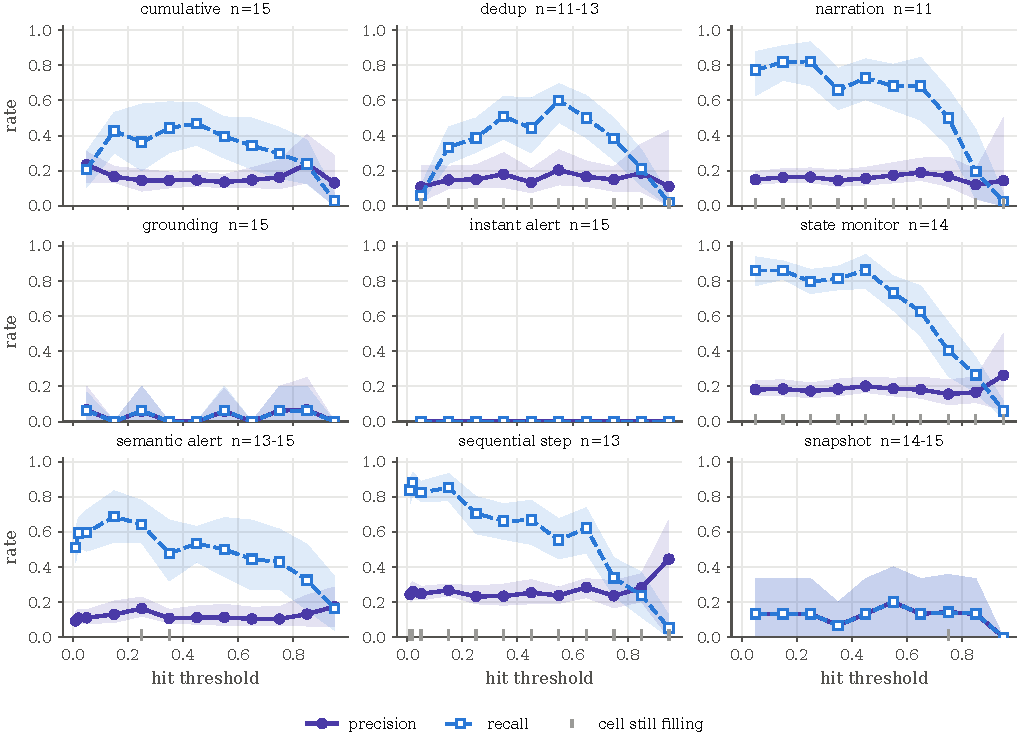
\includegraphics[width=0.92\linewidth]{../figs/fig3_pr_bands.pdf}
\caption{Precision--recall across the threshold grid with bootstrap bands. Precision is flat while recall falls: the threshold controls how \emph{often} the system speaks, not \emph{which moments} it picks.}\label{fig:pr}\end{figure}


\subsection{Finding 4 --- the fit does not survive its own bootstrap}

Pass 1 completed and \texttt{pick.py} returned a winner for all nine
tasks. A \emph{paired} bootstrap over the frozen videos --- same video set across
thresholds, and replaying \texttt{pick.rank} itself rather than a bare argmax ---
shows that \textbf{every task's $\Delta$F1 against its best rival has a 95\% CI
containing zero}, and that the fitted threshold is re-selected in only a minority
of draws (Table~\ref{tab:noise}). One task is re-selected \emph{below} its own
chance rate.

Two of the nine ``fits'' are artefacts and are labelled as such rather
than quietly reported: \texttt{instant\_event\_alert} scores 0.000 at every
threshold, which \texttt{pick.py} correctly flags \textsc{flat} while keeping the
shipped value; and \texttt{explicit\_target\_grounding}'s entire curve is one
matched event or zero out of 16, giving it the widest interval in the table. The
only reproducible structure anywhere in the sweep is the collapse at 0.95 --- the
threshold controls emission \emph{volume}, which is Finding 3 arriving again by a
different route.

\textbf{A prediction I recorded in advance was wrong.} Finding 3 led me
to predict that the fit would pin to the low rail on every task that emits.
It did not --- the picks scattered mid-grid. The reasoning error is recorded in
the runbook alongside the corrected prediction, because a prediction that is
quietly dropped after it fails is not a prediction.

\begin{table}[t]\centering\small\caption{Paired bootstrap over the 15 frozen videos, 2000 draws, resampling \emph{videos} (never ticks or events -- they are serially correlated through one shared KV cache). \emph{rival} is the best cell that is not the fitted one. \emph{re-sel.} re-runs \texttt{pick.rank} inside every draw and counts how often the fitted threshold wins again; compare it to chance, not to zero.}\label{tab:noise}
\begin{tabular}{lrrrlcrr}\toprule
task & fitted & rival & $\Delta$F1 & 95\% CI & CI$\ni$0 & re-sel. & chance \\\midrule
cumulative\_counting & 0.85 & 0.15 & +0.0013 & [-0.117, +0.137] & \textbf{yes} & 44\% & 10\% \\
dedup\_counting & 0.35 & 0.55 & -0.0174 & [-0.077, +0.034] & \textbf{yes} & 25\% & 10\% \\
event\_narration & 0.65 & 0.15 & +0.0023 & [-0.038, +0.043] & \textbf{yes} & 60\% & 10\% \\
explicit\_target\_grounding & 0.05 & 0.85 & -0.0022 & [-0.207, +0.182] & \textbf{yes} & 25\% & 10\% \\
instant\_event\_alert & 0.05 & 0.15 & +0.0000 & [+0.000, +0.000] & \textbf{yes} & 100\% & 10\% \\
realtime\_state\_monitor & 0.45 & 0.15 & +0.0179 & [-0.021, +0.057] & \textbf{yes} & 58\% & 10\% \\
semantic\_condition\_alert & 0.25 & 0.15 & -0.0183 & [-0.059, +0.021] & \textbf{yes} & 6\% & 8\% \\
sequential\_step\_instruction & 0.15 & 0.02 & +0.0141 & [-0.027, +0.046] & \textbf{yes} & 61\% & 8\% \\
snapshot\_counting & 0.55 & 0.05 & +0.0667 & [-0.133, +0.333] & \textbf{yes} & 28\% & 10\% \\
\bottomrule\end{tabular}\end{table}


\begin{figure}[t]\centering
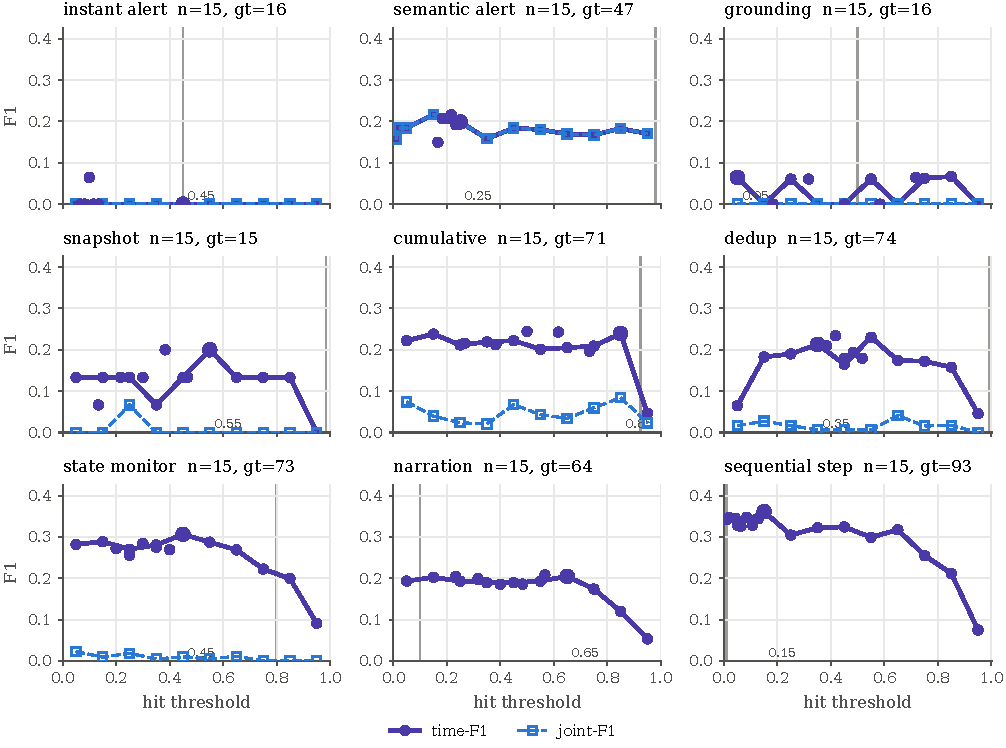
\includegraphics[width=0.92\linewidth]{../figs/fig1_f1_vs_threshold.pdf}
\caption{Time-F1 against threshold per task. Flat within the noise band across most of the grid, with the collapse at 0.95 the only consistent feature.}\label{fig:f1}\end{figure}


\subsection{Finding 5 --- one identifiable degree of freedom, not nine}

Four gate configurations were compared at equal budget on the same
videos, with a paired bootstrap over videos (Table~\ref{tab:ablation}). The nine
fitted thresholds beat the single best global threshold by an amount whose
interval straddles zero --- \emph{in sample}, where the fitted arm has nine free
parameters against the global arm's one.

Yet the global threshold itself is solid. Because
\texttt{best\_single\_global} is also an argmax over the same grid and the same
videos, it carries the identical winner's curse Finding 4 measured, so the entire
sweep is re-run inside every bootstrap draw. The value $0.15$ is re-selected in
\textbf{94\%} of draws against a chance rate of 10\%, versus the far lower
rates in Table~\ref{tab:noise} for the per-task fits.

\textbf{The thesis, stated carefully:} pooled over 135 videos the
operating point is identified; split nine ways over 15 videos each it is not.
That is a statement about statistical power, \emph{not} a claim that the nine
tasks are identical or that per-task gating cannot help. The shipped per-task
configuration is meanwhile significantly \emph{worse} than a flat global
threshold, and the mechanism is visible in the columns: it loses on recall, not
precision.

\begin{table}[t]\centering\small\caption{Gate ablation at equal budget, pooled over all 135 frozen videos and micro-averaged the way \texttt{metrics.aggregate} pools tp/fp/fn -- never a mean of per-sample ratios. $\Delta$ is against the best single global threshold, with a paired bootstrap CI over videos. \textbf{Caveat:} the grid does not contain every arm's threshold, so some cells are served by the nearest grid point (global 0.50: 9/9; shipped per-task: 7/9); every substitution is recorded in \texttt{ABLATION.json}.}\label{tab:ablation}
\begin{tabular}{lrrrl}\toprule
arm & time-P & time-R & time-F1 & $\Delta$ vs.\ BSG \\\midrule
global 0.50 & 0.1421 & 0.5650 & 0.2271 & -0.020 [-0.039, -0.003] \\
\textbf{best single global (0.15)} & 0.1554 & 0.6013 & 0.2469 & --- (reference) \\
shipped per-task & 0.1505 & 0.3561 & 0.2115 & -0.035 [-0.055, -0.016] \\
fitted per-task & 0.1628 & 0.5821 & 0.2544 & +0.007 [-0.011, +0.027] \\
\bottomrule\end{tabular}\end{table}


\begin{figure}[t]\centering
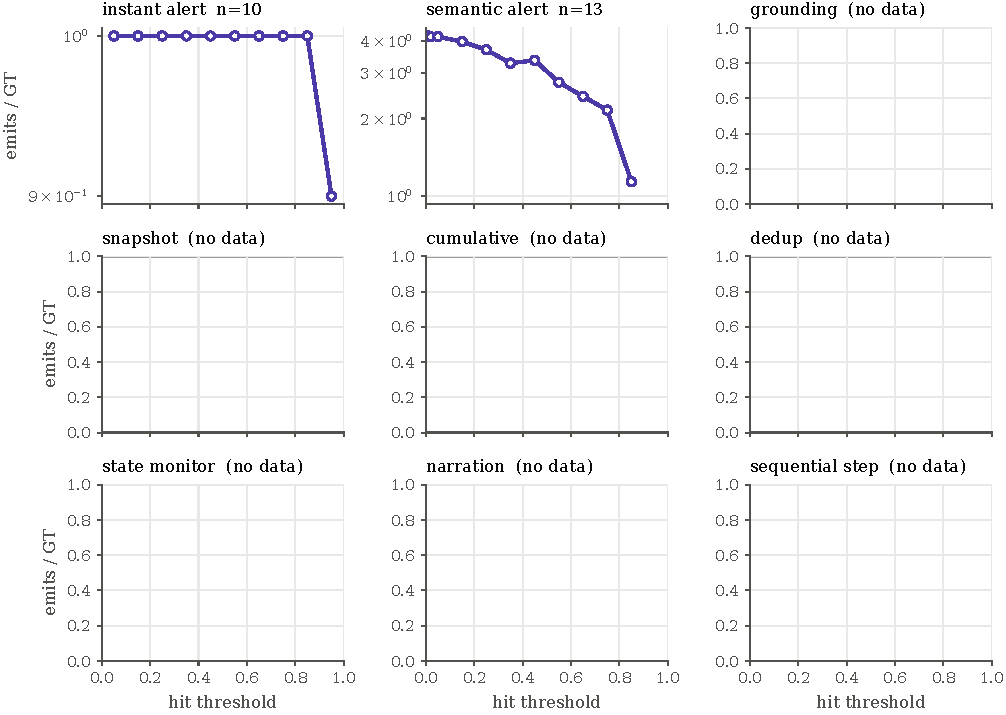
\includegraphics[width=0.92\linewidth]{../figs/fig4_emission_calibration.pdf}
\caption{Emissions per ground-truth event against threshold. The gate is a volume control: this curve is steep and orderly even where F1 is flat.}\label{fig:calib}\end{figure}


\subsection{Finding 6 --- pass 2 confirms a prediction registered in advance}

Pass 2 refined the grid around each pass-1 pick and completed
675/675 samples across 45/45 cells, every cell reliable. Before it finished, and
in writing, Finding 4 registered a prediction: that the refined grid's
$\Delta$F1-vs-rival intervals would contain zero on \emph{at least seven of
nine} tasks. \textbf{The outcome is 9 of 9} (Table~\ref{tab:noise2}). Recording
the prediction first is what makes this a test rather than a description.

\textbf{Two rows must be read carefully.} \texttt{instant\_event\_alert}
and \texttt{snapshot\_counting} report an interval of $[+0.000, +0.200]$. The
lower bound is exactly zero, so these \emph{do not} exclude it; both tasks match
0--2 events out of 15--16, and the interval is two grid-quantised jumps wide.
Calling that ``excludes zero'' would misread an inclusive bound as a tight
positive effect.

\textbf{The re-selection rates look better than pass 1's and are
not.} They read 38--74\% against pass 1's 25--61\%, but chance here is 20\% (five
cells per task) against 8--10\% there (ten to twelve). As a multiple of chance,
pass 2 runs 1.9--3.7$\times$ where pass 1 ran 2.5--6.1$\times$ --- no better, and
worse on four tasks. A finer grid packs cells closer together, making the argmax
\emph{less} separable, not more. Re-selection rates from grids of different sizes
must be divided by chance before they can be compared at all.

\textbf{What pass 2 genuinely adds is the span column.} Across each
refined neighbourhood the entire F1 range is 0.021--0.133, and on four of nine
tasks \emph{every} cell sits within the 0.03 noise band of the best. Refining the
grid did not resolve a winner; it confirmed there was no gradient there to
resolve --- Finding 3 arriving a fourth time by a fourth independent route.

\begin{table}[t]\centering\small\caption{Pass-2 paired bootstrap on the refined grid, same protocol as Table~\ref{tab:noise}. \emph{span} is the full F1 range across the task's refined neighbourhood; compare it against the 0.03 noise band. \emph{chance} is 20\% here because the refined grid has five cells per task, so re-selection rates are \textbf{not} comparable to Table~\ref{tab:noise}'s without dividing by it. Chance re-selection is 20\% on every task here (five cells each).}\label{tab:noise2}
\begin{tabular}{lrrrlcrr}\toprule
task & fitted & rival & $\Delta$F1 & 95\% CI & CI$\ni$0 & re-sel. & span \\\midrule
cumulative\_counting & 0.62 & 0.50 & -0.0017 & [-0.075, +0.085] & \textbf{yes} & 48\% & 0.048 \\
dedup\_counting & 0.42 & 0.38 & +0.0243 & [-0.025, +0.074] & \textbf{yes} & 70\% & 0.055 \\
event\_narration & 0.57 & 0.23 & +0.0037 & [-0.027, +0.031] & \textbf{yes} & 74\% & 0.022 \\
explicit\_target\_grounding & 0.72 & 0.32 & +0.0039 & [-0.182, +0.194] & \textbf{yes} & 47\% & 0.065 \\
instant\_event\_alert & 0.10 & 0.07 & +0.0645 & [+0.000, +0.200] & \textbf{yes} & 63\% & 0.065 \\
realtime\_state\_monitor & 0.35 & 0.30 & -0.0093 & [-0.033, +0.020] & \textbf{yes} & 38\% & 0.029 \\
semantic\_condition\_alert & 0.22 & 0.18 & +0.0091 & [-0.027, +0.061] & \textbf{yes} & 42\% & 0.066 \\
sequential\_step\_instruction & 0.09 & 0.04 & +0.0025 & [-0.027, +0.033] & \textbf{yes} & 41\% & 0.021 \\
snapshot\_counting & 0.38 & 0.22 & +0.0667 & [+0.000, +0.200] & \textbf{yes} & 56\% & 0.133 \\
\bottomrule\end{tabular}\end{table}


\begin{table}[t]\centering\small\caption{Final per-task thresholds. The selection ranks the pass-2 cells \emph{together with} the two pass-1 candidates, so a coarse point can still win --- which is why two finals are not on the pass-2 grid. A task flagged \textsc{flat} in pass 1 keeps its shipped value rather than being assigned a winner the data does not support.}\label{tab:final}
\begin{tabular}{lrrrl}\toprule
task & shipped & final & $\Delta$ & note \\\midrule
cumulative\_counting & 0.925 & 0.6167 & -0.308 &  \\
dedup\_counting & 0.992 & 0.5500 & -0.442 &  \\
event\_narration & 0.100 & 0.6500 & +0.550 &  \\
explicit\_target\_grounding & 0.500 & 0.7167 & +0.217 &  \\
instant\_event\_alert & 0.450 & 0.4500 & +0.000 & kept (flat) \\
realtime\_state\_monitor & 0.800 & 0.4500 & -0.350 &  \\
semantic\_condition\_alert & 0.980 & 0.2167 & -0.763 &  \\
sequential\_step\_instruction & 0.010 & 0.1500 & +0.140 &  \\
snapshot\_counting & 0.985 & 0.3833 & -0.602 &  \\
\bottomrule\end{tabular}\end{table}


Table~\ref{tab:final} is the artefact stage 3 would consume. The
selection ranks the pass-2 cells together with the two pass-1 candidates, so a
coarse point can win the finalise: two of the nine finals are not on the pass-2
grid at all, and one task keeps its shipped value because pass 1 flagged its
curve flat. Where the audit's fitted threshold is not a cell that was actually
run, it falls back to the rule's own pick on the pass-2 grid --- the alternative
would be scoring a cell that does not exist.

\textbf{One prediction remains open}, and it is the one that
matters: that on the held-out 2{,}700-sample stage-3 run, time-F1 under these
thresholds will land within the 0.03 noise band of the same run under the shipped
ones. That comparison is fit-disjoint, and it --- not the fit's own cells --- is
the arbiter of whether any of this fitting was real.

\section{Pass-1 selections}

Table~\ref{tab:picks} is the raw output of the selection rule, kept in
the report even though Finding 4 shows the individual picks are not resolvable.
It is the input that stage 3 would consume, and the negative result is only
legible next to the numbers it negates.

\begin{table}[t]\centering\small\caption{Pass-1 selection per task. \emph{gap} is best minus runner-up time-F1; a negative gap means sec.3's tie-band moved the pick off the raw argmax onto the emission volume closer to the truth. \textsc{flat} marks a task whose curve is identical at every threshold, where \texttt{pick.py} keeps the shipped value rather than inventing a winner.}\label{tab:picks}
\begin{tabular}{lrrrrrrl}\toprule
task & shipped & best & F1 & 2nd & gap & final & flags \\\midrule
cumulative\_counting & 0.925 & 0.85 & 0.2394 & 0.15 & +0.0013 & 0.85 & -- \\
dedup\_counting & 0.992 & 0.35 & 0.2132 & 0.55 & -0.0173 & 0.35 & -- \\
event\_narration & 0.100 & 0.65 & 0.2045 & 0.15 & +0.0023 & 0.65 & -- \\
explicit\_target\_grounding & 0.500 & 0.05 & 0.0645 & 0.85 & -0.0022 & 0.05 & rail \\
instant\_event\_alert & 0.450 & 0.05 & 0.0000 & 0.15 & +0.0000 & 0.45 & FLAT, rail \\
realtime\_state\_monitor & 0.800 & 0.45 & 0.3062 & 0.15 & +0.0179 & 0.45 & -- \\
semantic\_condition\_alert & 0.980 & 0.25 & 0.1986 & 0.15 & -0.0183 & 0.25 & -- \\
sequential\_step\_instruction & 0.010 & 0.15 & 0.3612 & 0.02 & +0.0141 & 0.15 & -- \\
snapshot\_counting & 0.985 & 0.55 & 0.2000 & 0.05 & +0.0667 & 0.55 & -- \\
\bottomrule\end{tabular}\end{table}


\section{Infrastructure and profiling}

The run tree is deliberately separate from the source repository so that
no run ever mutates the code under test, and it carries its own copy of the
interpreter, the weights cache and the dataset. That separation was not
precautionary theatre: mid-sweep, a \texttt{pip} reinstall of torch inside a
shared environment owned by another account changed 594 files and deleted
\texttt{torch/bin/torch\_shm\_manager}, and \texttt{import torch} failed outright
on every lane. Anything under another account's scratch can move without warning,
and the dataset case is worse than the environment case because it fails
\emph{silently} rather than loudly.

\textbf{Two fleets run in parallel.} The \texttt{debug} partition
allows at most 4 nodes and enforces a quota of 90 node-minutes per job, which
yields 4 nodes for 22 minutes, 2 for 45, or 1 for 90; only one job may run at a
time, with one more queued. The login nodes carry 4 GPUs each and are shared with
other users, so the fleet reads its GPU allocation from a file
(\texttt{LOGIN\_GPUS}) that can be changed while it runs.

\textbf{Every long job is self-chaining.} The wall-clock kill is a
SIGKILL, so nothing at the end of a script is guaranteed to execute; each
generation therefore pre-queues its successor with
\texttt{--dependency=afterany} \emph{before} doing any work. Resume is global
rather than per-lane, via a glob over the banked predictions, because the chain
reshapes 4$\to$2$\to$1 nodes and the lane count changes the shard assignment.

\textbf{Two scheduling defects were found and fixed by this run.}
First, a lane could re-claim the same barren shard for its whole window: the
scheduler returns the first incomplete claimable unit, and a shard whose samples
are all longer than the lane's remaining time is incomplete forever. That
produced 26{,}277 claims across seven generations --- all for one task --- while
84 of 94 cells were never touched. There are now two filters, one for barren
cells and one for barren shards, which the cell-level check cannot see. Second,
the chain read its worklist from a value baked in at first submit, one dropped
\texttt{--export} away from silently falling back to pass 1, finding it already
complete, and standing down looking like a finished run. The active pass is now
read from a file on every generation.

\textbf{Ordering hazard.} The subset stride selects by \emph{index}, so
any filter that shortens the sample list must be applied \emph{after} it; applied
before, it re-indexes the stride onto different samples. Measured cost of getting
this backwards: 487 of 688 evaluated ids landed outside the intended subset.

\textbf{Observed tail behaviour.} Completion is not uniform across
tasks (Table~\ref{tab:p2tail}) because a lane can only claim a shard whose
samples fit inside its remaining wall-clock. Late in a pass the outstanding
samples are the longest videos, the short-window debug lanes report every unit
barren, and the tail is carried almost entirely by the login lanes, which run
without a per-unit duration cap. This is expected rather than a fault, but it
means the last few percent of a pass proceed at a small fraction of its average
rate, and any schedule estimate that extrapolates the average will be wrong.

\section{What remains}

\begin{enumerate}
\item Finish pass 2, then \texttt{score\_cells}, \texttt{pick.py} and the
      bootstrap audit on it. All three are CPU-only and cost no GPU time. This
      tests a prediction registered in advance: that at least seven of the nine
      confidence intervals will again contain zero.
\item Apply the fitted thresholds and run stage 3, the full 2{,}700-sample
      evaluation. This is the bulk of the remaining compute.
\item Re-run the perception audit against stage 3, where it has $n=300$ per task
      instead of 15, and redraw the ROC figure from those logs.
\item Restore an LLM judge and lift the \WITHHELD{} on the content metrics. Three
      endpoints were tried and all failed --- one returning 404, one rate-limited,
      one unavailable.
\end{enumerate}

\textbf{Open decision.} Stage 3 cost scales with the number of gate arms
carried into it. Two arms --- the fitted per-task gate and the single best global
threshold --- is the recommendation: it is the comparison the report actually
turns on, and the wider ablation can stay on the fit subset where it already has
an answer.

\section{Reproducibility}

Every finding in this report regenerates from committed artefacts with
no GPU. The banked predictions are versioned --- they represent roughly 150
GPU-hours and the whole study is re-scorable from them offline --- while the
per-tick run logs are not, being large and reproducible by any re-run. Four
things live outside the repository and must be re-provided before any \emph{new}
sample can be evaluated: the benchmark manifest and its video corpus, the model
weights, the Python environment, and the working copy of the system under test.
Resume is keyed on the banked predictions, so nothing already completed is ever
recomputed.

\end{document}